% Options for packages loaded elsewhere
\PassOptionsToPackage{unicode}{hyperref}
\PassOptionsToPackage{hyphens}{url}
\PassOptionsToPackage{dvipsnames,svgnames,x11names}{xcolor}
%
\documentclass[
  letterpaper,
  DIV=11,
  numbers=noendperiod]{scrartcl}

\usepackage{amsmath,amssymb}
\usepackage{iftex}
\ifPDFTeX
  \usepackage[T1]{fontenc}
  \usepackage[utf8]{inputenc}
  \usepackage{textcomp} % provide euro and other symbols
\else % if luatex or xetex
  \usepackage{unicode-math}
  \defaultfontfeatures{Scale=MatchLowercase}
  \defaultfontfeatures[\rmfamily]{Ligatures=TeX,Scale=1}
\fi
\usepackage{lmodern}
\ifPDFTeX\else  
    % xetex/luatex font selection
\fi
% Use upquote if available, for straight quotes in verbatim environments
\IfFileExists{upquote.sty}{\usepackage{upquote}}{}
\IfFileExists{microtype.sty}{% use microtype if available
  \usepackage[]{microtype}
  \UseMicrotypeSet[protrusion]{basicmath} % disable protrusion for tt fonts
}{}
\makeatletter
\@ifundefined{KOMAClassName}{% if non-KOMA class
  \IfFileExists{parskip.sty}{%
    \usepackage{parskip}
  }{% else
    \setlength{\parindent}{0pt}
    \setlength{\parskip}{6pt plus 2pt minus 1pt}}
}{% if KOMA class
  \KOMAoptions{parskip=half}}
\makeatother
\usepackage{xcolor}
\setlength{\emergencystretch}{3em} % prevent overfull lines
\setcounter{secnumdepth}{5}
% Make \paragraph and \subparagraph free-standing
\ifx\paragraph\undefined\else
  \let\oldparagraph\paragraph
  \renewcommand{\paragraph}[1]{\oldparagraph{#1}\mbox{}}
\fi
\ifx\subparagraph\undefined\else
  \let\oldsubparagraph\subparagraph
  \renewcommand{\subparagraph}[1]{\oldsubparagraph{#1}\mbox{}}
\fi


\providecommand{\tightlist}{%
  \setlength{\itemsep}{0pt}\setlength{\parskip}{0pt}}\usepackage{longtable,booktabs,array}
\usepackage{calc} % for calculating minipage widths
% Correct order of tables after \paragraph or \subparagraph
\usepackage{etoolbox}
\makeatletter
\patchcmd\longtable{\par}{\if@noskipsec\mbox{}\fi\par}{}{}
\makeatother
% Allow footnotes in longtable head/foot
\IfFileExists{footnotehyper.sty}{\usepackage{footnotehyper}}{\usepackage{footnote}}
\makesavenoteenv{longtable}
\usepackage{graphicx}
\makeatletter
\def\maxwidth{\ifdim\Gin@nat@width>\linewidth\linewidth\else\Gin@nat@width\fi}
\def\maxheight{\ifdim\Gin@nat@height>\textheight\textheight\else\Gin@nat@height\fi}
\makeatother
% Scale images if necessary, so that they will not overflow the page
% margins by default, and it is still possible to overwrite the defaults
% using explicit options in \includegraphics[width, height, ...]{}
\setkeys{Gin}{width=\maxwidth,height=\maxheight,keepaspectratio}
% Set default figure placement to htbp
\makeatletter
\def\fps@figure{htbp}
\makeatother

\usepackage{booktabs}
\usepackage{longtable}
\usepackage{array}
\usepackage{multirow}
\usepackage{wrapfig}
\usepackage{float}
\usepackage{colortbl}
\usepackage{pdflscape}
\usepackage{tabu}
\usepackage{threeparttable}
\usepackage{threeparttablex}
\usepackage[normalem]{ulem}
\usepackage{makecell}
\usepackage{xcolor}
\setlength{\tabcolsep}{1pt}
\usepackage{fontspec}
\usepackage{fontawesome}
\usepackage{endfloat}
\usepackage{pdflscape}
\setlength{\tabcolsep}{2pt}
\DeclareDelayedFloatFlavour*{longtable}{table}
\DeclareDelayedFloatFlavor{landscape}{table}
\KOMAoption{captions}{tableheading}
\makeatletter
\makeatother
\makeatletter
\makeatother
\makeatletter
\@ifpackageloaded{caption}{}{\usepackage{caption}}
\AtBeginDocument{%
\ifdefined\contentsname
  \renewcommand*\contentsname{Table of contents}
\else
  \newcommand\contentsname{Table of contents}
\fi
\ifdefined\listfigurename
  \renewcommand*\listfigurename{List of Figures}
\else
  \newcommand\listfigurename{List of Figures}
\fi
\ifdefined\listtablename
  \renewcommand*\listtablename{List of Tables}
\else
  \newcommand\listtablename{List of Tables}
\fi
\ifdefined\figurename
  \renewcommand*\figurename{Figure}
\else
  \newcommand\figurename{Figure}
\fi
\ifdefined\tablename
  \renewcommand*\tablename{Table}
\else
  \newcommand\tablename{Table}
\fi
}
\@ifpackageloaded{float}{}{\usepackage{float}}
\floatstyle{ruled}
\@ifundefined{c@chapter}{\newfloat{codelisting}{h}{lop}}{\newfloat{codelisting}{h}{lop}[chapter]}
\floatname{codelisting}{Listing}
\newcommand*\listoflistings{\listof{codelisting}{List of Listings}}
\makeatother
\makeatletter
\@ifpackageloaded{caption}{}{\usepackage{caption}}
\@ifpackageloaded{subcaption}{}{\usepackage{subcaption}}
\makeatother
\makeatletter
\@ifpackageloaded{tcolorbox}{}{\usepackage[skins,breakable]{tcolorbox}}
\makeatother
\makeatletter
\@ifundefined{shadecolor}{\definecolor{shadecolor}{rgb}{.97, .97, .97}}
\makeatother
\makeatletter
\makeatother
\makeatletter
\makeatother
\ifLuaTeX
  \usepackage{selnolig}  % disable illegal ligatures
\fi
\usepackage[authoryear,longnamesfirst]{natbib}
\bibliographystyle{plainnat}
\IfFileExists{bookmark.sty}{\usepackage{bookmark}}{\usepackage{hyperref}}
\IfFileExists{xurl.sty}{\usepackage{xurl}}{} % add URL line breaks if available
\urlstyle{same} % disable monospaced font for URLs
\hypersetup{
  pdftitle={Manuscript methods and results},
  pdfauthor={Matthew Andreotta; Fabio Boschetti; Simon Farrell; Cécile Paris; Iain Walker; Mark Hurlstone},
  colorlinks=true,
  linkcolor={blue},
  filecolor={Maroon},
  citecolor={Blue},
  urlcolor={Blue},
  pdfcreator={LaTeX via pandoc}}

\title{Manuscript methods and results}
\author{Matthew Andreotta \and Fabio Boschetti \and Simon
Farrell \and Cécile Paris \and Iain Walker \and Mark Hurlstone}
\date{2024-09-27}

\begin{document}
\maketitle
\ifdefined\Shaded\renewenvironment{Shaded}{\begin{tcolorbox}[interior hidden, breakable, borderline west={3pt}{0pt}{shadecolor}, boxrule=0pt, frame hidden, enhanced, sharp corners]}{\end{tcolorbox}}\fi

\hypertarget{summary}{%
\section{Summary}\label{summary}}

This document contains the methods and results for the manuscript.

\hypertarget{methods}{%
\section{Methods}\label{methods}}

Data and analysis scripts for the study are available online at
\url{https://github.com/matt-lab/bushfire-audience-segmentation}. This
study was approved by the Human Research Ethics Committees of the
University of Western Australia (reference: 2019/RA/4/20/5104) and the
Commonwealth Scientific and Industrial Research Organisation (reference:
026/19).

\hypertarget{participants-and-design}{%
\subsection{Participants and design}\label{participants-and-design}}

The study was a longitudinal design, where data was collected at three
time periods, as presented in Table~\ref{tbl-waves}. Study 1 was
conducted before in September (\textit{n} = 387, 88.97\% of
participants), October (\textit{n} = 42, 9.66\% of participants), and
November (\textit{n} = 6, 1.38\% of participants) of 2019 prior to the
peak severity of the Black Summer bushfires. Study 2, conducted in
February (\textit{n} = 403, 97.58\% of participants) and March
(\textit{n} = 10, 2.42\% of participants) of 2020, and Study 3,
conducted in March of 2020 (\textit{n} = 213), were both completed after
the peak severity of the Black Summer bushfires. In total, 1061
Australian adults participated in the study. Participants were recruited
complete an online survey via Qualtrics---an Internet panel services
platform. We used a targeted and stratified sampling process was used to
match the age and gender of each studies' sample to the general
population (as per the national 2016 census). We discarded the data of
extremely fast responders, who were categorised using a preregistered
threshold (see Supplementary Materials).

\hypertarget{tbl-waves}{}
\begin{table}
\caption{\label{tbl-waves}Sample characteristics and materials of study. }\tabularnewline

\centering
\begin{tabular}[t]{>{\raggedright\arraybackslash}p{16em}>{\centering\arraybackslash}p{7em}>{\centering\arraybackslash}p{7em}>{\centering\arraybackslash}p{7em}}
\toprule
\multicolumn{1}{c}{ } & \multicolumn{3}{c}{Study} \\
\cmidrule(l{3pt}r{3pt}){2-4}
Characteristics & 1 & 2 & 3\\
\midrule
Time & Before peak bushfire severity & After peak bushfire severity & After peak bushfire severity\\
\addlinespace[0.3em]
\multicolumn{4}{l}{\textbf{Data collection dates}}\\
\hspace{1em}Start & 24-SEP-2019 & 25-FEB-2020 & 13-MAR-2020\\
\hspace{1em}End & 09-NOV-2019 & 02-MAR-2020 & 26-MAR-2020\\
\addlinespace[0.3em]
\multicolumn{4}{l}{\textbf{Sample characteristics}}\\
\hspace{1em}\textit{n} & 435 & 413 & 213\\
\hspace{1em}Mean age in years (\textit{SD}) & 46.71 (17.77) & 46.82 (18.04) & 47.13 (17.29)\\
\hspace{1em}Number of women in sample (\%) & 213 (48.97\%) & 206 (49.88\%) & 107 (50.23\%)\\
\addlinespace[0.3em]
\multicolumn{4}{l}{\textbf{Materials}}\\
\hspace{1em}Q-sort & \faCheck & \faCheck & \faCheck\\
\hspace{1em}Auxiliary psychological scales & \faCheck & \faClose & \faCheck\\
\hspace{1em}Fire Perception Scale & \faClose & \faClose & \faCheck\\
\hspace{1em}Change in policy items & \faClose & \faClose & \faCheck\\
\bottomrule
\end{tabular}
\end{table}

\hypertarget{materials}{%
\subsection{Materials}\label{materials}}

Psychological inventories and tasks were used to gauge climate change
and bushfire perceptions, in addition to auxiliary psychological
characteristics.

\hypertarget{q-sort}{%
\subsubsection{Q-sort}\label{q-sort}}

To measure climate change views, we used the Q-sort. The Q-sort is a
card-sorting task, where participants ranked thirty cards with climate
change statements, such as ``it is important to vote for leaders who
will combat climate change'' and ``scientists should stop falsely
claiming that climate change is a settled science''. The statements were
selected to reflect the breadth of the Australian climate change
discourse on social media \citep{andreotta_2022}. To encourage
reflection, participants began the Q-sort by reading each card and
determining if the statement was: (1) like their point of view; (2)
unlike their point of view; or neutral or unsure. Next, participants
ranked their relative agreement for each statement by assigning ranks to
each statement, from -4 (most unlike their point of view) through to +4
(most like their point of view). The distribution of possible ranks is
forced and non-uniform, such that participants must consider the few
statements to place at the extremes (see Figure~\ref{fig-qsort}). This
encourages participants to carefully reflect on their views whilst
completing the task \citep{stephenson1986, brown1980}. Following
completion of the survey, participants were asked to justify their
placement of statements ranked most extreme.

\begin{figure}

{\centering 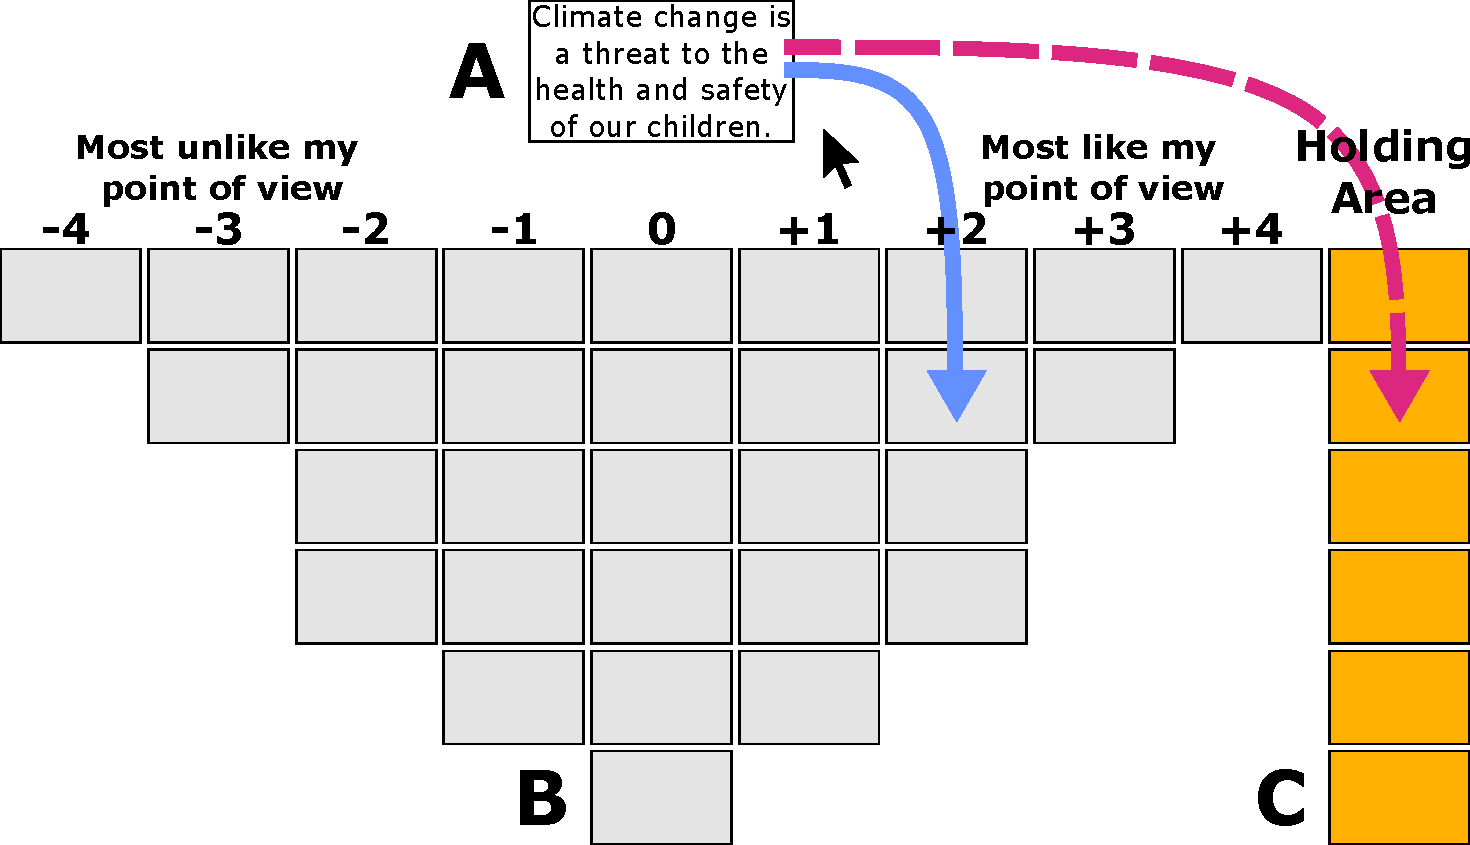
\includegraphics[width=1\textwidth,height=\textheight]{qsort.pdf}

}

\caption{\label{fig-qsort}Schematic of the Q-sort task. Participants
read through a stack of statements (A) by dragging the top-most
statement into the grey box that best corresponded to their point of
view (B). As the majority of statements had to be placed around the
midpoint, participants could only highlight a few statements that
strongly reflect their point of view. Participants could re-arrange
statements at any time during the task. To facilitate this process,
participants could temporarily place statements in the yellow holding
area (C). Figure reproduced without changes from \citep{andreotta_2022},
under the Creative Commons license (CC BY 4.0).}

\end{figure}

\hypertarget{auxiliary-psychological-scales}{%
\subsubsection{Auxiliary psychological
scales}\label{auxiliary-psychological-scales}}

In Study 1 and Study 3, we quantified twenty-eight auxiliary
psychological characteristics (Table~\ref{tbl-scales}).

Most relevant to the current research were climate change cognition and
affect inventories. We measured general belief in anthropogenic climate
change, with scales concerning epistemic scepticism (doubt concerning
anthropogenic climate change), response scepticism (doubt concerning the
effectiveness of climate change mitigation), perceived human
contribution (belief that humans have changed global climate), knowledge
volume (self-perceived confidence in climate change knowledge), and
worry about climate change. In addition, we included higher-resolution
inventories to quantify participants mental models of specific climate
change causes, consequences, and effectiveness of climate change
mitigation policies.

Other psychological scales pertained to trait-based concepts found to be
associated with climate change belief. This includes inventories
concerning: cognitive styles; ideology, worldviews, and values; and
personality.

\hypertarget{tbl-scales}{}
\begin{landscape}\begingroup\fontsize{7}{9}\selectfont

\begin{longtable}[t]{>{\raggedright\arraybackslash}p{20em}>{\raggedright\arraybackslash}p{3.5em}>{\raggedright\arraybackslash}p{6em}>{\raggedright\arraybackslash}p{3.5em}>{\raggedright\arraybackslash}p{30em}>{\raggedright\arraybackslash}p{13em}}
\caption{\label{tbl-scales}Summary of auxiliary psychological measures. }\tabularnewline

\toprule
Psychological characteristic & Items & Cronbach's $\alpha$ & Range & Example item & Reference\\
\midrule
\endfirsthead
\multicolumn{6}{@{}l}{\textit{(continued)}}\\
\toprule
Psychological characteristic & Items & Cronbach's $\alpha$ & Range & Example item & Reference\\
\midrule
\endhead

\endfoot
\bottomrule
\multicolumn{6}{l}{\rule{0pt}{1em}\textit{Note: }}\\
\multicolumn{6}{l}{\rule{0pt}{1em}\parbox{70em}{Conservation and Self-Transcendence Value scores were a weighted average of ten items (rated along a nine-point scale). Table reproduced with updated Cronbach's $\alpha$ from \citet{andreotta_2022}, under the Creative Commons license (CC BY 4.0).}}\\
\endlastfoot
\addlinespace[0.3em]
\multicolumn{6}{l}{\textbf{Climate change cognition and affect}}\\
\hspace{1em}Knowledge Volume & 1 & - & 1 to 4 & How much do you feel you know about climate change? & \citet{malka2009}\\
\hspace{1em}Perceptions of Carbon Emission Causes & 7 & 0.92 & 1 to 7 & Please indicate to what extent each of the following is a cause of climate change, to the best of your knowledge: people driving their cars & \citet{andreotta_2022}\\
\hspace{1em}Perceptions of Environmental Harm Causes & 4 & 0.87 & 1 to 7 & Please indicate to what extent each of the following is a cause of climate change, to the best of your knowledge: air pollution from toxic chemicals & \citet{andreotta_2022}\\
\hspace{1em}Perceptions of Natural Causes & 2 & 0.79 & 1 to 7 & Please indicate to what extent each of the following is a cause of climate change, to the best of your knowledge: volcanic eruptions & \citet{andreotta_2022}\\
\hspace{1em}Perceived Personal Consequences & 3 & 0.87 & 1 to 7 & Please rate for each of the following how likely it is as a consequence of climate change by the year 2050: food shortages where you live & \citet{bostrom2012}\\
\hspace{1em}Perceived Societal Consequences & 8 & 0.96 & 1 to 7 & Please rate for each of the following how likely it is as a consequence of climate change by the year 2050: food shortages in many parts of the world & \citet{bostrom2012}\\
\hspace{1em}Perceived Human Contribution & 1 & - & 1 to 7 & How likely do you think it is that human actions have changed global climate? & \citet{bostrom2012}\\
\hspace{1em}Perceived Effectiveness of Carbon Policies & 3 & 0.75 & 1 to 7 & Please rate for each step what effect you think it would have on climate change: requiring cars and trucks to have higher fuel efficiency (1 = Reduce or Stop Climate Change, 4 = Neither Reduce nor Increase, 7 = Increase Climate Change) & \citet{bostrom2012}\\
\hspace{1em}Perceived Effectiveness of Engineering Policies & 3 & 0.42 & 1 to 7 & Please rate for each step what effect you think it would have on climate change: putting more dust in the atmosphere (1 = Reduce or Stop Climate Change, 4 = Neither Reduce nor Increase, 7 = Increase Climate Change) & \citet{bostrom2012}\\
\hspace{1em}Perceived Effectiveness of Green Policies & 5 & 0.91 & 1 to 7 & Please rate for each step what effect you think it would have on climate change: planting trees (1 = Reduce or Stop Climate Change, 4 = Neither Reduce nor Increase, 7 = Increase Climate Change) & \citet{bostrom2012}\\
\hspace{1em}Epistemic Scepticism & 8 & 0.91 & 1 to 5 & Climate change is just a natural fluctuation in Earth's temperatures & \citet{capstick2014}\\
\hspace{1em}Response Scepticism & 7 & 0.89 & 1 to 5 & There is no point in me doing anything about climate change because no-one else is & \citet{capstick2014}\\
\hspace{1em}Worry about Climate Change & 1 & - & 1 to 4 & How strongly do you feel worry when you think about the issue of climate change? & \citet{smith2014}\\
\addlinespace[0.3em]
\multicolumn{6}{l}{\textbf{Cognitive style}}\\
\hspace{1em}Orientation to Future Goals & 4 & 0.72 & 1 to 5 & I consider how things might be in the future & \citet{enzler2015}\\
\hspace{1em}Orientation to Immediate Goals & 5 & 0.86 & 1 to 5 & I mainly act to satisfy my immediate concerns, figuring the future will take care of itself & \citet{enzler2015}\\
\hspace{1em}Conspiracist Ideation & 6 & 0.90 & 1 to 5 & The Apollo moon landings never happened and were staged in a Hollywood film studio & \citet{lewandowsky2013}\\
\hspace{1em}Need for Cognition & 6 & 0.79 & 1 to 5 & I would prefer complex to simple problems & \citet{linsdeholandacoelho2018}\\
\addlinespace[0.3em]
\multicolumn{6}{l}{\textbf{Ideology, worldviews, or values}}\\
\hspace{1em}Environment-as-Ductile Worldview & 6 & 0.81 & 1 to 5 & If the balance of the natural environment is upset the whole system will collapse & \citet{price2014}\\
\hspace{1em}Environment-as-Elastic Worldview & 6 & 0.85 & 1 to 5 & The natural environment is capable of recovering from any damage humans may cause & \citet{price2014}\\
\hspace{1em}Political Ideology & 1 & - & 1 to 7 & Please indicate the extent to which you identify yourself as politically left-wing or right-wing (1 = Very Left-Wing, 7 = Very Right-Wing) & -\\
\hspace{1em}System Justification & 8 & 0.85 & 1 to 9 & Everyone has a fair shot at wealth and happiness & \citet{kay2003}\\
\hspace{1em}Conservation Values & 10 & 0.32 & -2.94 to 5.54 & Please, rate the importance of the following values as a life-guiding principle for you: CONFORMITY (obedience, honouring parents and elders, self-discipline, politeness) & \citet{lindeman2005}\\
\hspace{1em}Self-Transcendence Values & 10 & 0.55 & -4.84 to 2.52 & Please, rate the importance of the following values as a life-guiding principle for you: BENEVOLENCE (helpfulness, honesty, forgiveness, loyalty, responsibility) & \citet{lindeman2005}\\
\addlinespace[0.3em]
\multicolumn{6}{l}{\textbf{Personality}}\\
\hspace{1em}Agreeableness & 2 & 0.27 & 1 to 5 & I see myself as someone who is generally trusting & \citet{rammstedt2007}\\
\hspace{1em}Conscientiousness & 2 & 0.53 & 1 to 5 & I see myself as someone who does a thorough job & \citet{rammstedt2007}\\
\hspace{1em}Extraversion & 2 & 0.53 & 1 to 5 & I see myself as someone who is outgoing, sociable & \citet{rammstedt2007}\\
\hspace{1em}Neuroticism & 2 & 0.62 & 1 to 5 & I see myself as someone who gets nervous easily & \citet{rammstedt2007}\\
\hspace{1em}Openness & 2 & 0.14 & 1 to 5 & I see myself as someone who has an active imagination & \citet{rammstedt2007}\\*
\end{longtable}
\endgroup{}
\end{landscape}

\hypertarget{fire-perception-scale}{%
\subsubsection{Fire Perception Scale}\label{fire-perception-scale}}

To measure perceptions of the Black Summer bushfires, we created a Fire
Perception Scale. The scale's seven items were constructed from
prominent media and politicians' statements on the role of climate
change in Black Summer. Items included ``climate change made the 2019-20
Australian bushfires more severe'' and ``over one hundred arsonists have
contributed to the 2019-20 Australian bushfires''. Participants respond
on a five-point Likert scale: (1) disagree, (2) slightly disagree, (3)
neither agree nor disagree, (4) slightly agree, and (5) agree.

\hypertarget{policy-direction-preferences}{%
\subsubsection{Policy direction
preferences}\label{policy-direction-preferences}}

To measure participants views on the policy consequences of the Black
Summer bushfires, we asked participants to respond to two items. First,
participants were asked: ``Do the 2019-20 Australian bushfires justify a
change in Australia's climate change policy?''. Participants could
respond with one of four options: (1) ``yes, the Australian government
should be taking further action to mitigate climate change''; (2) ``no,
the Australian government should not modify the current climate change
policy''; (3) ``yes, the Australian government should be taking less
action to mitigate climate change''; and (4) ``yes, the Australian
government should be taking no action at all to mitigate climate
change''. Next, participants were asked to justify their response
(``Why?'') through writing an open-ended response.

\hypertarget{procedure}{%
\subsection{Procedure}\label{procedure}}

All studies began with the same procedure. To begin, participants read
an information sheet, provided informed consent, and provided
demographic information. Next, procedure varied across studies
(summarised in Table~\ref{tbl-waves}). In Study 1, participants
completed the Q-sort followed by the auxiliary psychological scales. In
Study 2, participants completed the Q-sort followed by a task unrelated
to our current research inquiry. In Study 3, participants completed all
materials: the Q-sort, auxiliary psychological scales, the Fire
Perception Scale, and policy direction preferences. The presentation
sequence of materials were counterbalanced across participants to
control for order effects (see Supplementary Materials).

\hypertarget{results}{%
\section{Results}\label{results}}

All analyses were completed with the \emph{R} programming language
\citep{rcoreteam_2023}.

\hypertarget{replication-of-the-three-segment-solution}{%
\subsection{Replication of the three-segment
solution}\label{replication-of-the-three-segment-solution}}

As per our previous research, we used the Q-methodology to identify
distinct views on climate change \citep{brown1980}. The Q-methodology
transposes traditional dimension reduction techniques, to reduce the
dimensions of \emph{people} rather than \emph{items}. For each study, we
used principal components analysis with varimax rotation to group
individuals with similar Q-sort ranks. We extracted a single factor, as
the first component accounted for a large portion of variance than
subsequent components for each study. This single factor represented a
dimension of anthropogenic climate change acceptance. Based on factor
loadings, we divided individuals into one of three segments: (1)
\emph{Acceptors} (\(n = 653\), 61.55\%), whose positive factor loading
was statistically significant from zero (\(p < .05\)); (2)
\emph{Sceptics} (\(n = 97\), 9.14\%), whose negative factor loading was
statistically significant from zero (\(p < .05\)); and (3)
\emph{Fencesitters} (\(n = 311\), 29.31\%), whose factor loading was not
statistically significant from zero (\(p \ge .05\)).

Although the number of segments was consistent across studies, the
nature of segments may vary. To explore this possibility, we constructed
an average Q-sort for Acceptors and Sceptics in each study
\citep{brown1980}. The ranks assigned to each statement were averaged
(weighted by participants' factor loading). These averages are then
ranked to be consistent with Q-sort structure, to produce a set of
numbers known as factor scores. For example, the statement with the
lowest average was assigned a factor score of -4 and the statement with
the highest average was assigned a factor score of +4 (see Supplementary
Material for all factor scores). We did not build a representative
Q-sort for Fencesitters, as point estimates cannot represent the
necessarily homogeneous segment (otherwise Fencesitters would have
emerged as a separate factor). In all three studies, the greatest factor
score for Acceptors was assigned to the statement ``It is important to
vote for leaders who will combat climate change'' whereas the greatest
factor score for Sceptics was assigned to the statement ``Scientists
should stop falsely claiming that climate change is a settled science.''

We found minimal differences in each segment's factor scores across
studies Acceptor factor ranks from the three studies were strongly
correlated (all Spearman's \(\rho\) correlations \(> 0.95\), all \(p\)'s
\(< .001\)). Likewise, Sceptic factor ranks across studies were strongly
correlated (all Spearman's \(\rho\) correlations \(> 0.94\), all \(p\)'s
\(< .001\)). Consistently across studies, Acceptors and Sceptics views
held divergent views (all Spearman's \(\rho\) correlations \(< -0.81\),
all \(p\)'s \(< .001\)). In sum, the number and nature of segments were
consistent across time.

\hypertarget{change-in-segment-membership-over-time}{%
\subsection{Change in segment membership over
time}\label{change-in-segment-membership-over-time}}

To explore whether segment membership changed during Black Summer, we
investigated the relative proportions of segments across studies
(Figure~\ref{fig-segment-change}). Numerically, the proportion of
Acceptors fell across time (from 64.60\% of Study 1 sample to 54.46\% of
Study 3 sample), whereas the proportion of Fencesitters increased across
time (from 27.13\% of Study 1 sample to 37.09\% of Study 3 sample). To
investigate whether these changes were statistically significant, we
created a multinomial logistic regression model to predict segment
membership as a function of study (coefficients reported in
Supplementary Material), using the \emph{multinom} function from the
\emph{nnet} package \citep{venables_2002}. A log likelihood ratio test
did not indicate an improvement in model fit when study was included as
a predictor, compared to a model with only an intercept term
(\(\chi^{2}\) (4) = 8.85, \(p\) = 0.07). Thus, segment membership did
not reliably differ across study samples.

\begin{figure}

{\centering 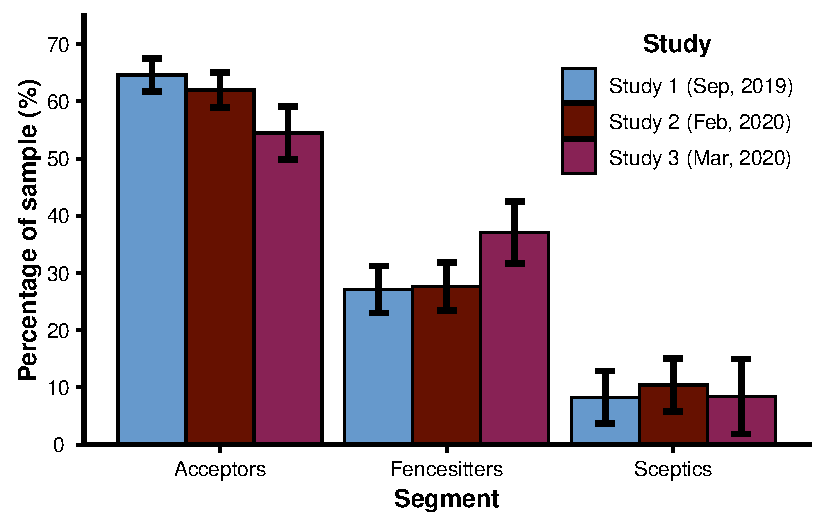
\includegraphics{analysis_files/figure-pdf/fig-segment-change-1.pdf}

}

\caption{\label{fig-segment-change}The segment membership of each
study's sample, as a proportion (percentage). Error bars indicate one
standard error of the proportion.}

\end{figure}

\hypertarget{auxiliary-psychological-characteristics}{%
\subsection{Auxiliary psychological
characteristics}\label{auxiliary-psychological-characteristics}}

We tested for mean differences in auxiliary psychological
characteristics between Study 1 (September, 2019) and Study 3 (March,
2020) using \emph{t} tests. To guard against Type I errors, we applied a
Holm \citeyearpar{holm1979} \emph{p} value adjustment to four families
of tests for changes in psychological characteristics: climate change
cognition and affect; cognitive styles; ideology, worldviews, and
values; and personality. We found evidence of a statistically
significant mean difference in climate change cognition and affect
(Table~\ref{tbl-mean_diff}). Specifically, participants in Study 3 had a
greater mean endorsement (Cohen's \emph{d} = 0.25) of natural cycles
causes for climate change (e.g., volcanic eruptions, fluctuations in the
sun) than participants of Study 1. No other climate change cognition and
affect characteristics reliably differed between Study 1 and Study 3.
Regarding dispositional attributes, there were no statistically
significant mean differences in: cognitive styles; ideology, worldviews
and values; or personality (all \(p\) \textgreater{} .05; see
Supplementary Material for \emph{t} tests).

\hypertarget{tbl-mean_diff}{}
\begin{table}
\caption{\label{tbl-mean_diff}Difference in means of climate change cognition and affect
characteristics between Study 1 and Study 3. }\tabularnewline

\centering
\begin{tabular}[t]{l>{\raggedright\arraybackslash}p{5em}>{\raggedright\arraybackslash}p{5em}>{\raggedright\arraybackslash}p{2.5em}>{\raggedright\arraybackslash}p{3em}>{\raggedright\arraybackslash}p{4em}}
\toprule
\multicolumn{1}{c}{ } & \multicolumn{1}{c}{\parbox{4em}{Study 1}} & \multicolumn{1}{c}{\parbox{4em}{Study 3}} & \multicolumn{3}{c}{ } \\
\cmidrule(l{3pt}r{3pt}){2-2} \cmidrule(l{3pt}r{3pt}){3-3}
Psychological characteristics & \textit{M} (\textit{SD}) & \textit{M} (\textit{SD}) & \textit{t} & \textit{p} & $p_{adjusted}$\\
\midrule
Perceptions of Natural Causes & 4.23 (1.51) & 4.62 (1.62) & 2.95 & .003 & .044*\\
Response Scepticism & 2.37 (1.01) & 2.56 (0.99) & 2.29 & .022 & .269\\
Perceived Effectiveness of Green Policies & 4.69 (1.52) & 4.49 (1.50) & -1.60 & .110 & 1.000\\
Worry about Climate Change & 2.72 (1.01) & 2.61 (1.01) & -1.35 & .178 & 1.000\\
Perceptions of Carbon Emission Causes & 5.06 (1.33) & 4.91 (1.40) & -1.29 & .197 & 1.000\\
Perceived Human Contribution & 5.59 (1.72) & 5.41 (1.71) & -1.22 & .222 & 1.000\\
Epistemic Scepticism & 2.97 (1.00) & 3.05 (0.99) & 1.04 & .300 & 1.000\\
Knowledge Volume & 2.69 (0.76) & 2.76 (0.78) & 0.99 & .325 & 1.000\\
Perceived Personal Consequences & 4.59 (1.58) & 4.71 (1.40) & 0.97 & .331 & 1.000\\
Perceptions of Environmental Harm Causes & 4.61 (1.49) & 4.51 (1.57) & -0.75 & .457 & 1.000\\
Perceived Effectiveness of Engineering Policies & 4.04 (1.06) & 4.00 (1.08) & -0.43 & .670 & 1.000\\
Perceived Effectiveness of Carbon Policies & 4.19 (1.26) & 4.15 (1.32) & -0.33 & .742 & 1.000\\
Perceived Societal Consequences & 5.12 (1.51) & 5.10 (1.41) & -0.11 & .914 & 1.000\\
\bottomrule
\multicolumn{6}{l}{\rule{0pt}{1em}\textit{Note: }}\\
\multicolumn{6}{l}{\rule{0pt}{1em}\textsuperscript{*}$p_{adjusted} <$ .05; }\\
\multicolumn{6}{l}{\rule{0pt}{1em}\parbox{36em}{\textit{p} values were adjusted using the \citet{holm1979} method.}}\\
\end{tabular}
\end{table}

We explored the psychological characteristics associated with segment
membership, by replicating the regression analysis of Andreotta et al.
\citeyearpar{andreotta_2022}. This analysis is complicated by
multicollinearity, which can lead to unstable estimates of coefficients.
We sought to produce stable estimates with a ridge regression model. A
ridge regression reduces the variance of estimates, caused by
multicollinearity, by shrinking the coefficients towards zero {[}a
bias-variance trade-off; \citet{james_2021}{]}. With the \emph{glmnet}
package \citep{friedman_2010}, we fitted a multinomial logistic ridge
regression model to predict segment membership as a function of
psychological characteristics for Study 1 and Study 3. The degree of
shrinkage, controlled by a hyperparameter \(\lambda\), was chosen by
cross-validation process (\emph{k}-fold) that minimised the model's
multinomial deviance. Prior to analysis, we converted responses to
\emph{z} scores for each predictor in each study. Confidence intervals
were estimated by repeating the modelling procedure via bootstrapping
with 10,000 samples {[}sampled with replacement; \citet{efron1994}{]}.

The ridge regression model predicted segment membership with 83.22\%
accuracy in Study 1 (49.07\% of null deviance) and 88.26\% accuracy in
Study 3 (66.39 \% of null deviance). As seen in
Table~\ref{tbl-ridge-regression-segments-within-studies}, the models'
coefficients were generally consistent (same sign) across studies,
indicating a robust association between psychological characteristics
and segment membership. Regarding climate change cognition and affect,
Acceptors and Sceptics were distinguished by opposing patterns of
climate change scepticism and belief in anthropogenic climate change. In
contrast, the Fencesitters of Study 3 were characterised by response
scepticism and perceptions that carbon-emitting activities cause climate
change. Turning to cognitive styles, conspiracist ideation was
positively associated with Fencesitter membership, and negatively
associated with Acceptor membership (both studies), whereas Sceptics
were characterised by a reduced orientation towards future consequences
(Study 3). Generally, Acceptors and Sceptics were distinguished by
opposing patterns of ideologies, worldviews, and values. Lastly,
personality tended not to be a robust predictor of segment membership,
although evidence from Study 3 indicated that Fencesitters were
characterised by greater extraversion and conscientiousness, whereas
Sceptics were characterised by greater introversion.

\hypertarget{tbl-ridge-regression-segments-within-studies}{}
\begin{landscape}\begingroup\fontsize{7}{9}\selectfont

\begin{longtable}[t]{>{\raggedright\arraybackslash}p{20em}>{\raggedright\arraybackslash}p{8em}>{\raggedright\arraybackslash}p{8em}>{\raggedright\arraybackslash}p{8em}>{\raggedright\arraybackslash}p{8em}>{\raggedright\arraybackslash}p{8em}l}
\caption{\label{tbl-ridge-regression-segments-within-studies}Effect of psychological characteristics on segment membership, as
estimated by a multinomial logistic ridge regression for Study 1 and
Study 3. }\tabularnewline

\toprule
\multicolumn{1}{c}{ } & \multicolumn{2}{c}{Acceptors} & \multicolumn{2}{c}{Fencesitters} & \multicolumn{2}{c}{Sceptics} \\
\cmidrule(l{3pt}r{3pt}){2-3} \cmidrule(l{3pt}r{3pt}){4-5} \cmidrule(l{3pt}r{3pt}){6-7}
Predictors & Study 1 & Study 3 & Study 1 & Study 3 & Study 1 & Study 3\\
\midrule
\endfirsthead
\multicolumn{7}{@{}l}{\textit{(continued)}}\\
\toprule
\multicolumn{1}{c}{ } & \multicolumn{2}{c}{Acceptors} & \multicolumn{2}{c}{Fencesitters} & \multicolumn{2}{c}{Sceptics} \\
\cmidrule(l{3pt}r{3pt}){2-3} \cmidrule(l{3pt}r{3pt}){4-5} \cmidrule(l{3pt}r{3pt}){6-7}
Predictors & Study 1 & Study 3 & Study 1 & Study 3 & Study 1 & Study 3\\
\midrule
\endhead

\endfoot
\bottomrule
\multicolumn{7}{l}{\rule{0pt}{1em}\textit{Note: }}\\
\multicolumn{7}{l}{\rule{0pt}{1em}\parbox{70em}{Square brackets indicate 95\% confidence intervals, estimated using bootstrapping with 10,000 samples. Coefficients with confidence intervals that do not include zero are marked with a caret (textasciicircum) and are bolded.}}\\
\endlastfoot
\addlinespace[0.3em]
\multicolumn{7}{l}{\textbf{Intercept}}\\
\hspace{1em} & \parbox{7em}{\textbf{+1.64\textasciicircum\\{[1.64, 2.18]}}} & \parbox{7em}{\textbf{+1.66\textasciicircum\\{[1.44, 2.09]}}} & \parbox{7em}{\textbf{+0.56\textasciicircum\\{[0.44, 0.99]}}} & \parbox{7em}{\textbf{+1.03\textasciicircum\\{[0.71, 1.32]}}} & \parbox{7em}{\textbf{-2.20\textasciicircum\\{[-3.06, -2.19]}}} & \parbox{7em}{\textbf{-2.69\textasciicircum\\{[-3.22, -2.36]}}}\\
\addlinespace[0.3em]
\multicolumn{7}{l}{\textbf{Climate change cognition and affect}}\\
\hspace{1em}Epistemic Scepticism & \parbox{7em}{\textbf{-0.33\textasciicircum\\{[-0.59, -0.26]}}} & \parbox{7em}{\textbf{-0.46\textasciicircum\\{[-0.72, -0.25]}}} & \parbox{7em}{+0.11\\{[-0.05, 0.30]}} & \parbox{7em}{+0.13\\{[-0.08, 0.39]}} & \parbox{7em}{\textbf{+0.23\textasciicircum\\{[0.16, 0.43]}}} & \parbox{7em}{\textbf{+0.33\textasciicircum\\{[0.19, 0.46]}}}\\
\hspace{1em}Worry about Climate Change & \parbox{7em}{\textbf{+0.31\textasciicircum\\{[0.23, 0.60]}}} & \parbox{7em}{+0.13\\{[-0.09, 0.38]}} & \parbox{7em}{-0.06\\{[-0.25, 0.11]}} & \parbox{7em}{+0.10\\{[-0.12, 0.36]}} & \parbox{7em}{\textbf{-0.25\textasciicircum\\{[-0.50, -0.19]}}} & \parbox{7em}{\textbf{-0.23\textasciicircum\\{[-0.44, -0.07]}}}\\
\hspace{1em}Response Scepticism & \parbox{7em}{\textbf{-0.29\textasciicircum\\{[-0.55, -0.19]}}} & \parbox{7em}{\textbf{-0.55\textasciicircum\\{[-0.75, -0.37]}}} & \parbox{7em}{+0.08\\{[-0.09, 0.28]}} & \parbox{7em}{\textbf{+0.34\textasciicircum\\{[0.14, 0.56]}}} & \parbox{7em}{\textbf{+0.21\textasciicircum\\{[0.15, 0.40]}}} & \parbox{7em}{\textbf{+0.21\textasciicircum\\{[0.09, 0.35]}}}\\
\hspace{1em}Perceived Human Contribution & \parbox{7em}{\textbf{+0.20\textasciicircum\\{[0.08, 0.41]}}} & \parbox{7em}{\textbf{+0.27\textasciicircum\\{[0.12, 0.51]}}} & \parbox{7em}{+0.12\\{[-0.02, 0.35]}} & \parbox{7em}{-0.06\\{[-0.29, 0.16]}} & \parbox{7em}{\textbf{-0.32\textasciicircum\\{[-0.59, -0.23]}}} & \parbox{7em}{\textbf{-0.22\textasciicircum\\{[-0.42, -0.07]}}}\\
\hspace{1em}Perceived Societal Consequences & \parbox{7em}{\textbf{+0.19\textasciicircum\\{[0.06, 0.39]}}} & \parbox{7em}{+0.11\\{[-0.08, 0.38]}} & \parbox{7em}{-0.09\\{[-0.30, 0.05]}} & \parbox{7em}{+0.06\\{[-0.21, 0.25]}} & \parbox{7em}{-0.10\\{[-0.23, 0.04]}} & \parbox{7em}{\textbf{-0.16\textasciicircum\\{[-0.33, -0.02]}}}\\
\hspace{1em}Perceptions of Environmental Harm Causes & \parbox{7em}{+0.08\\{[-0.09, 0.26]}} & \parbox{7em}{+0.04\\{[-0.18, 0.24]}} & \parbox{7em}{+0.08\\{[-0.08, 0.28]}} & \parbox{7em}{+0.19\\{[0.00, 0.43]}} & \parbox{7em}{\textbf{-0.16\textasciicircum\\{[-0.32, -0.05]}}} & \parbox{7em}{\textbf{-0.22\textasciicircum\\{[-0.37, -0.10]}}}\\
\hspace{1em}Knowledge Volume & \parbox{7em}{-0.10\\{[-0.34, 0.01]}} & \parbox{7em}{-0.05\\{[-0.25, 0.13]}} & \parbox{7em}{-0.06\\{[-0.24, 0.10]}} & \parbox{7em}{-0.01\\{[-0.22, 0.19]}} & \parbox{7em}{\textbf{+0.15\textasciicircum\\{[0.04, 0.43]}}} & \parbox{7em}{+0.06\\{[-0.11, 0.26]}}\\
\hspace{1em}Perceptions of Carbon Emission Causes & \parbox{7em}{\textbf{+0.15\textasciicircum\\{[0.00, 0.35]}}} & \parbox{7em}{+0.15\\{[-0.02, 0.32]}} & \parbox{7em}{+0.04\\{[-0.11, 0.23]}} & \parbox{7em}{\textbf{+0.29\textasciicircum\\{[0.09, 0.49]}}} & \parbox{7em}{\textbf{-0.19\textasciicircum\\{[-0.36, -0.11]}}} & \parbox{7em}{\textbf{-0.44\textasciicircum\\{[-0.59, -0.29]}}}\\
\hspace{1em}Perceived Effectiveness of Engineering Policies & \parbox{7em}{\textbf{-0.13\textasciicircum\\{[-0.36, -0.01]}}} & \parbox{7em}{+0.09\\{[-0.11, 0.31]}} & \parbox{7em}{\textbf{+0.14\textasciicircum\\{[0.01, 0.36]}}} & \parbox{7em}{-0.10\\{[-0.31, 0.11]}} & \parbox{7em}{-0.01\\{[-0.14, 0.15]}} & \parbox{7em}{+0.01\\{[-0.15, 0.16]}}\\
\hspace{1em}Perceived Personal Consequences & \parbox{7em}{+0.12\\{[-0.03, 0.30]}} & \parbox{7em}{+0.12\\{[-0.09, 0.36]}} & \parbox{7em}{-0.02\\{[-0.19, 0.14]}} & \parbox{7em}{-0.09\\{[-0.31, 0.15]}} & \parbox{7em}{-0.10\\{[-0.23, 0.02]}} & \parbox{7em}{-0.03\\{[-0.21, 0.11]}}\\
\hspace{1em}Perceived Effectiveness of Carbon Policies & \parbox{7em}{+0.11\\{[-0.03, 0.35]}} & \parbox{7em}{-0.13\\{[-0.34, 0.09]}} & \parbox{7em}{-0.03\\{[-0.23, 0.15]}} & \parbox{7em}{+0.17\\{[-0.07, 0.36]}} & \parbox{7em}{-0.08\\{[-0.27, 0.02]}} & \parbox{7em}{-0.03\\{[-0.16, 0.13]}}\\
\hspace{1em}Perceived Effectiveness of Green Policies & \parbox{7em}{+0.10\\{[-0.02, 0.30]}} & \parbox{7em}{-0.04\\{[-0.24, 0.17]}} & \parbox{7em}{-0.04\\{[-0.20, 0.14]}} & \parbox{7em}{+0.10\\{[-0.12, 0.31]}} & \parbox{7em}{-0.06\\{[-0.27, 0.05]}} & \parbox{7em}{-0.06\\{[-0.20, 0.08]}}\\
\hspace{1em}Perceptions of Natural Causes & \parbox{7em}{-0.08\\{[-0.26, 0.08]}} & \parbox{7em}{-0.15\\{[-0.40, 0.05]}} & \parbox{7em}{+0.05\\{[-0.10, 0.24]}} & \parbox{7em}{+0.10\\{[-0.12, 0.36]}} & \parbox{7em}{+0.02\\{[-0.15, 0.20]}} & \parbox{7em}{+0.05\\{[-0.16, 0.25]}}\\
\addlinespace[0.3em]
\multicolumn{7}{l}{\textbf{Cognitive style}}\\
\hspace{1em}Orientation to Future Goals & \parbox{7em}{+0.05\\{[-0.11, 0.25]}} & \parbox{7em}{+0.21\\{[0.00, 0.38]}} & \parbox{7em}{+0.06\\{[-0.10, 0.26]}} & \parbox{7em}{+0.10\\{[-0.09, 0.30]}} & \parbox{7em}{-0.11\\{[-0.33, 0.04]}} & \parbox{7em}{\textbf{-0.31\textasciicircum\\{[-0.47, -0.11]}}}\\
\hspace{1em}Conspiracist Ideation & \parbox{7em}{\textbf{-0.15\textasciicircum\\{[-0.36, -0.02]}}} & \parbox{7em}{\textbf{-0.49\textasciicircum\\{[-0.70, -0.32]}}} & \parbox{7em}{\textbf{+0.15\textasciicircum\\{[0.02, 0.36]}}} & \parbox{7em}{\textbf{+0.33\textasciicircum\\{[0.15, 0.55]}}} & \parbox{7em}{+0.00\\{[-0.18, 0.17]}} & \parbox{7em}{+0.16\\{[-0.02, 0.34]}}\\
\hspace{1em}Need for Cognition & \parbox{7em}{-0.12\\{[-0.32, 0.01]}} & \parbox{7em}{-0.07\\{[-0.25, 0.15]}} & \parbox{7em}{+0.01\\{[-0.15, 0.18]}} & \parbox{7em}{-0.02\\{[-0.23, 0.19]}} & \parbox{7em}{+0.10\\{[-0.03, 0.31]}} & \parbox{7em}{+0.09\\{[-0.12, 0.27]}}\\
\hspace{1em}Orientation to Immediate Goals & \parbox{7em}{+0.02\\{[-0.12, 0.25]}} & \parbox{7em}{-0.16\\{[-0.42, 0.00]}} & \parbox{7em}{0.00\\{[-0.20, 0.17]}} & \parbox{7em}{+0.15\\{[-0.04, 0.41]}} & \parbox{7em}{-0.02\\{[-0.21, 0.10]}} & \parbox{7em}{+0.02\\{[-0.18, 0.21]}}\\
\addlinespace[0.3em]
\multicolumn{7}{l}{\textbf{Ideology, worldviews, and values}}\\
\hspace{1em}Environment-as-Ductile Worldview & \parbox{7em}{+0.18\\{[-0.01, 0.44]}} & \parbox{7em}{\textbf{+0.40\textasciicircum\\{[0.23, 0.62]}}} & \parbox{7em}{-0.11\\{[-0.36, 0.05]}} & \parbox{7em}{\textbf{-0.21\textasciicircum\\{[-0.43, -0.01]}}} & \parbox{7em}{-0.07\\{[-0.21, 0.10]}} & \parbox{7em}{\textbf{-0.19\textasciicircum\\{[-0.36, -0.04]}}}\\
\hspace{1em}Conservation Values & \parbox{7em}{-0.11\\{[-0.32, 0.02]}} & \parbox{7em}{\textbf{-0.26\textasciicircum\\{[-0.46, -0.06]}}} & \parbox{7em}{+0.01\\{[-0.17, 0.18]}} & \parbox{7em}{-0.02\\{[-0.22, 0.22]}} & \parbox{7em}{+0.11\\{[-0.05, 0.32]}} & \parbox{7em}{\textbf{+0.27\textasciicircum\\{[0.06, 0.45]}}}\\
\hspace{1em}Environment-as-Elastic Worldview & \parbox{7em}{\textbf{-0.20\textasciicircum\\{[-0.43, -0.05]}}} & \parbox{7em}{\textbf{-0.37\textasciicircum\\{[-0.58, -0.20]}}} & \parbox{7em}{+0.05\\{[-0.15, 0.23]}} & \parbox{7em}{+0.07\\{[-0.12, 0.33]}} & \parbox{7em}{\textbf{+0.15\textasciicircum\\{[0.03, 0.38]}}} & \parbox{7em}{\textbf{+0.30\textasciicircum\\{[0.12, 0.46]}}}\\
\hspace{1em}System Justification & \parbox{7em}{+0.04\\{[-0.12, 0.25]}} & \parbox{7em}{\textbf{+0.20\textasciicircum\\{[0.04, 0.39]}}} & \parbox{7em}{+0.06\\{[-0.12, 0.23]}} & \parbox{7em}{\textbf{-0.23\textasciicircum\\{[-0.44, -0.04]}}} & \parbox{7em}{-0.09\\{[-0.30, 0.07]}} & \parbox{7em}{+0.03\\{[-0.16, 0.22]}}\\
\hspace{1em}Self-Transcendence Values & \parbox{7em}{+0.04\\{[-0.10, 0.21]}} & \parbox{7em}{+0.17\\{[-0.04, 0.36]}} & \parbox{7em}{-0.10\\{[-0.28, 0.05]}} & \parbox{7em}{+0.02\\{[-0.20, 0.21]}} & \parbox{7em}{+0.06\\{[-0.12, 0.24]}} & \parbox{7em}{\textbf{-0.19\textasciicircum\\{[-0.33, 0.00]}}}\\
\hspace{1em}Political Ideology & \parbox{7em}{\textbf{-0.18\textasciicircum\\{[-0.41, -0.04]}}} & \parbox{7em}{-0.10\\{[-0.35, 0.12]}} & \parbox{7em}{+0.03\\{[-0.17, 0.19]}} & \parbox{7em}{-0.16\\{[-0.38, 0.06]}} & \parbox{7em}{\textbf{+0.16\textasciicircum\\{[0.02, 0.40]}}} & \parbox{7em}{\textbf{+0.26\textasciicircum\\{[0.09, 0.47]}}}\\
\addlinespace[0.3em]
\multicolumn{7}{l}{\textbf{Personality}}\\
\hspace{1em}Extraversion & \parbox{7em}{-0.01\\{[-0.15, 0.14]}} & \parbox{7em}{+0.03\\{[-0.21, 0.22]}} & \parbox{7em}{+0.03\\{[-0.11, 0.19]}} & \parbox{7em}{\textbf{+0.23\textasciicircum\\{[0.04, 0.45]}}} & \parbox{7em}{-0.02\\{[-0.18, 0.11]}} & \parbox{7em}{\textbf{-0.26\textasciicircum\\{[-0.43, -0.07]}}}\\
\hspace{1em}Conscientiousness & \parbox{7em}{+0.03\\{[-0.09, 0.20]}} & \parbox{7em}{-0.14\\{[-0.33, 0.01]}} & \parbox{7em}{-0.06\\{[-0.21, 0.09]}} & \parbox{7em}{\textbf{+0.19\textasciicircum\\{[0.01, 0.39]}}} & \parbox{7em}{+0.03\\{[-0.15, 0.16]}} & \parbox{7em}{-0.05\\{[-0.19, 0.11]}}\\
\hspace{1em}Neuroticism & \parbox{7em}{+0.11\\{[-0.01, 0.30]}} & \parbox{7em}{+0.03\\{[-0.15, 0.22]}} & \parbox{7em}{-0.02\\{[-0.17, 0.14]}} & \parbox{7em}{-0.08\\{[-0.30, 0.10]}} & \parbox{7em}{-0.09\\{[-0.29, 0.01]}} & \parbox{7em}{+0.05\\{[-0.09, 0.23]}}\\
\hspace{1em}Agreeableness & \parbox{7em}{+0.04\\{[-0.11, 0.20]}} & \parbox{7em}{+0.01\\{[-0.18, 0.24]}} & \parbox{7em}{+0.02\\{[-0.13, 0.17]}} & \parbox{7em}{-0.03\\{[-0.27, 0.16]}} & \parbox{7em}{-0.06\\{[-0.21, 0.10]}} & \parbox{7em}{+0.03\\{[-0.18, 0.23]}}\\
\hspace{1em}Openness & \parbox{7em}{0.00\\{[-0.16, 0.14]}} & \parbox{7em}{+0.01\\{[-0.18, 0.23]}} & \parbox{7em}{-0.07\\{[-0.24, 0.06]}} & \parbox{7em}{0.00\\{[-0.22, 0.19]}} & \parbox{7em}{+0.07\\{[-0.05, 0.25]}} & \parbox{7em}{-0.01\\{[-0.22, 0.17]}}\\*
\end{longtable}
\endgroup{}
\end{landscape}

\hypertarget{bushfire-perceptions}{%
\subsection{Bushfire perceptions}\label{bushfire-perceptions}}

To explore perceptions of the Black Summer bushfires, we performed a
principal components analysis with varimax rotation on the Fire
Perception Scale (see Table~\ref{tbl-fps-loadings}). We extracted three
factors, as these accounted for the majority of scale variance (78.31\%;
see Supplementary Materials for scree plot). The first factor, labelled
\emph{Climate Processes}, was characterised by four items (items 1, 3,
5, 6) which linked climate change to the bushfires and accounted for
41.22\% of scale variance. The second factor, labelled \emph{Fire
Realities}, was characterised by two items (items 2 and 4) which
participants generally responded with certainty and accounted for
19.97\% of scale variance. The third factor, labelled \emph{Arson
Causes}, was characterised by a single item (item 7) stating that Black
Summer was caused by hundreds of arsonists and accounted for 17.12\% of
scale variance. We created subscales corresponding to each factor by
averaging item scores. Items that negatively loaded onto factors were
reverse coded. The multi-item factors of Climate Processes and Fire
Realities had an internal consistency of Cronbach's \(\alpha\) = 0.86
and 0.42, respectively.

To test segment differences in bushfire perceptions, we built linear
regression models predicting Climate Processes, Fire Realities, and
Arson Causes as a function of segment membership (coefficients reported
in Supplementary Materials). All linear regression models accounted for
a significant amount of bushfire perception variance compared to
intercept-only models, indicating that segment membership was a
significant predictor of Climate Processes (\(F\) (2, 210) = 47.44,
\(p\) \textless{} .001, \(R^2\) = 0.31, \(R^2_{adjusted}\) = 0.30), Fire
Realities (\(F\) (2, 210) = 30.31, \(p\) \textless{} .001, \(R^2\) =
0.22, \(R^2_{adjusted}\) = 0.22), and Arson Causes (\(F\) (2, 210) =
12.69, \(p\) \textless{} .001, \(R^2\) = 0.11, \(R^2_{adjusted}\) =
0.10). To quantify specific segment differences, we conducted pairwise
comparisons of marginal means using the \emph{marginaleffects} package
\citep{R-marginaleffects}, with a Holm \citeyearpar{holm1979} \emph{p}
value adjustment for multiple comparisons. As seen in
Figure~\ref{fig-fps-segment}, Acceptors had a higher mean endorsement of
Climate Processes than Fencesitters (difference = 0.53, \emph{SE} =
0.14, \emph{z} = 3.87, \(p\) \textless{} .001, \(p_{adjusted}\)
\textless{} .001), who in turn, had a higher mean endorsement than
Sceptics (difference = 1.76, \emph{SE} = 0.25, \emph{z} = 7.14, \(p\)
\textless{} .001, \(p_{adjusted}\) \textless{} .001). For Fire
Realities, Acceptors had a greater mean endorsement than Sceptics
(difference = 0.48, \emph{SE} = 0.19, \emph{z} = 2.54, \(p\) = .011,
\(p_{adjusted}\) = .022) and Fencesitters (difference = 0.84, \emph{SE}
= 0.11, \emph{z} = 7.75, \(p\) \textless{} .001, \(p_{adjusted}\)
\textless{} .001). However, Fencesitters did not reliably differ from
Sceptics in their mean endorsement of Fire Realities (difference =
-0.36, \emph{SE} = 0.20, \emph{z} = -1.86, \(p\) = .063,
\(p_{adjusted}\) = .063). The pattern of Climate Processes endorsement
was reversed for Arson Causes, with Sceptics having a higher mean
endorsement than Fencesitters (difference = 0.74, \emph{SE} = 0.30,
\emph{z} = 2.47, \(p\) = .014, \(p_{adjusted}\) = .014), who in turn,
had a higher mean endorsement than Acceptors (difference = 0.55,
\emph{SE} = 0.17, \emph{z} = 3.32, \(p\) \textless{} .001,
\(p_{adjusted}\) = .002).

\hypertarget{tbl-fps-loadings}{}
\begin{table}
\caption{\label{tbl-fps-loadings}Items of the Fire Perception Scale, their loadings onto each factor, the
mean score of each item, and the standard error of the mean. }\tabularnewline

\centering
\begin{tabular}[t]{>{\raggedright\arraybackslash}p{18em}ccccc}
\toprule
\multicolumn{1}{c}{ } & \multicolumn{3}{c}{Factors} & \multicolumn{2}{c}{Descriptives} \\
\cmidrule(l{3pt}r{3pt}){2-4} \cmidrule(l{3pt}r{3pt}){5-6}
Item & \parbox{5em}{\centering Climate Processes} & \parbox{5em}{\centering Fire Realities} & \parbox{5em}{\centering Arson Causes} & \textit{M} & \textit{SE}\\
\midrule
1. Climate change made the 2019-20 Australian bushfires more severe & \textbf{0.78} & 0.34 & -0.22 & 3.62 & 0.10\\
2. Climate change made the 2019-20 Australian bushfires less likely to occur & 0.27 & \textbf{-0.70} & \textbf{0.42} & 2.19 & 0.09\\
3. The 2019-20 Australian bushfires have accelerated climate change & \textbf{0.84} & 0.05 & -0.14 & 3.16 & 0.09\\
4. The 2019-20 Australian bushfires are severe & 0.17 & \textbf{0.86} & 0.23 & 4.50 & 0.05\\
5. If the government increased taxes on all fossil fuels (e.g., gasoline, oil, coal, kerosene), Australia would be less likely to experience extreme bushfires & \textbf{0.84} & -0.19 & 0.13 & 2.55 & 0.09\\
6. If we changed our lifestyles to reduce our consumption, Australia would be less likely to experience bushfires & \textbf{0.86} & -0.06 & 0.08 & 3.05 & 0.09\\
7. Over one hundred arsonists have contributed to the 2019-20 Australian bushfires & -0.10 & 0.04 & \textbf{0.94} & 3.47 & 0.08\\
\bottomrule
\multicolumn{6}{l}{\rule{0pt}{1em}\textit{Note: }}\\
\multicolumn{6}{l}{\rule{0pt}{1em}Bolded loadings are greater than .40 in magnitude.}\\
\end{tabular}
\end{table}

\begin{figure}

{\centering 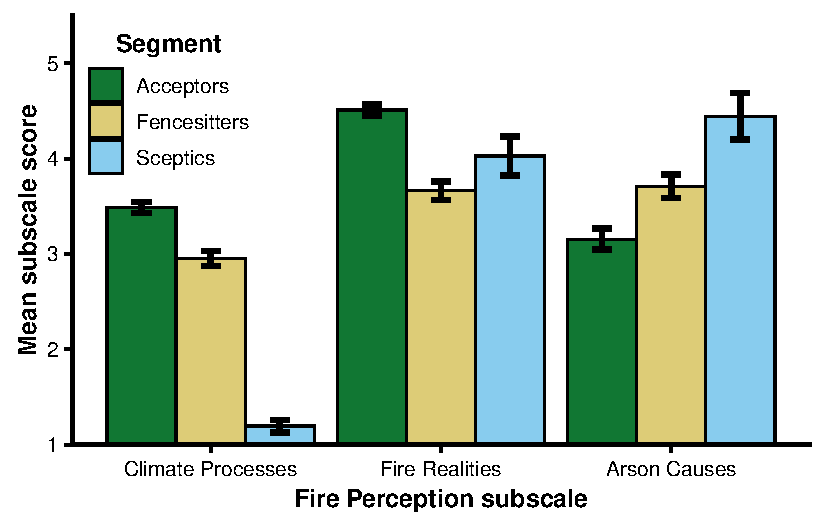
\includegraphics{analysis_files/figure-pdf/fig-fps-segment-1.pdf}

}

\caption{\label{fig-fps-segment}Mean Fire Perception subscale scores as
a function of segment. Error bars indicate one standard error above and
below the mean.}

\end{figure}

We investigated causal perceptions by examining responses to claims that
the mass arson (item seven of the Bushfire Perception scale) and climate
change (item one of the Bushfire Perception Scale) contributed to the
Black Summer bushfires. Despite segment differences, participants seldom
rejected the claim that over one hundred arsonists contributed to the
Black Summer bushfires (\emph{n} = 38; 17.84\% responded with `disagree'
or `strongly disagree' to item seven). Many Acceptors (\emph{n} = 45;
38.79\%), and a majority of Fencesitters (\emph{n} = 45; 56.96\%) and
Sceptics (\emph{n} = 16; 88.89\%), agreed (responded with `agree' or
`strongly agree') with mass arson causal claims. In contrast, a majority
of Acceptors (\emph{n} = 101; 87.07\%), some Fencesitters (\emph{n} =
33; 41.77\%), and no Sceptics agreed that climate change worsened the
Black Summer bushfires. Endorsement of the mass arson causal account was
negatively associated with endorsement of climate change causal account
(\emph{r} = -0.21, \emph{p} = .002), which suggests that the two causal
accounts for the Black Summer bushfires were somewhat incompatible.

\hypertarget{policy-direction-preferences-1}{%
\subsection{Policy direction
preferences}\label{policy-direction-preferences-1}}

Participants differed in their policy direction preferences in response
to the Black Summer bushfires. Most participants desired more
governmental climate change mitigation policies (\(n = 145\), 68.08\%),
or no changes to governmental climate change mitigation policies
(\(n = 54\), 25.35\%). Few participants desired less or no governmental
climate change mitigation policies (totalling \(n = 14\), 6.57\%).
Policy direction preferences differed across segments, with the majority
of Acceptors and Fencesitters desiring more governmental climate change
mitigation policies, and the majority of Sceptics desiring no changes to
governmental climate change mitigation policies
(Figure~\ref{fig-policy-support}). We investigated the statistical
significance of segment differences using a binomial logistic regression
model, estimated the odds of desiring more governmental climate change
mitigation policies as a function of segment membership (reported in
full in Supplementary Materials). Sceptics were excluded from analysis,
as none desired more governmental climate change mitigation policies. A
likelihood-ratio test indicated that segment membership significantly
predicted policy direction preferences (\(\chi^{2}\) (1) = 35.45, \(p\)
\textless{} .001). Specifically, we found that the odds of Acceptors
(\(n\) = 104, 89.66\% of Acceptors, odds = 8.67) indicating a preference
for more governmental climate change mitigation policies were
approximately eight times greater (odds ratio = 8.03, 95\% \emph{CI} =
{[}3.92, 17.49{]}, \(p\) \textless{} .001) than Fencesitters (\(n\) =
41, 51.90\% of Fencesitters, odds = 1.08).

We explored the text justification of policy direction preferences using
an emotion analysis. We detected the emotional association of each word
using the NRC Word-Emotion Association Lexicon \citep{mohammad_2013}.
This lexicon is a list of words manually annotated (via crowdsourcing)
for their association with eight emotions: anger, fear, anticipation,
trust, surprise, sadness, joy, and disgust. For each response, we
assigned a dichotomous code (present/not present) if the response
contained at least one word associated with an emotion, for each
emotion. The most common emotion evoked by participants was fear
(\(n = 67\), 31.46\%), found in both justification for more action
(``the recent bushfire is a wakupe call. how much more \emph{worse} do
we want to experience?'', fear words italicised) and for no changes or
less action (``\ldots100 arsonists were charged as a starter and the it
was the fuel left on the ground for decades that made the fires so much
\emph{worse} and caused the \emph{disaster}'', fear words italicised).
To test whether emotions varied across segments, we made a binomial
logistic regression model for each emotion with segment membership as a
predictor (reported in full in Supplementary Materials). Generally, we
found no statistically significant differences in the use of emotions
across segments, except for fear, where the odds of Acceptors using a
fear word (\(n\) = 47, 40.52\% of Acceptors, odds = 0.68) were
approximately three times higher (odds ratio = 3.16, 95\% \emph{CI} =
{[}1.59, 6.28{]}, \(p\) = .001) than Fencesitters (\(n\) = 14, 17.72\%
of Fencesitters, odds = 0.22).

\begin{figure}

{\centering 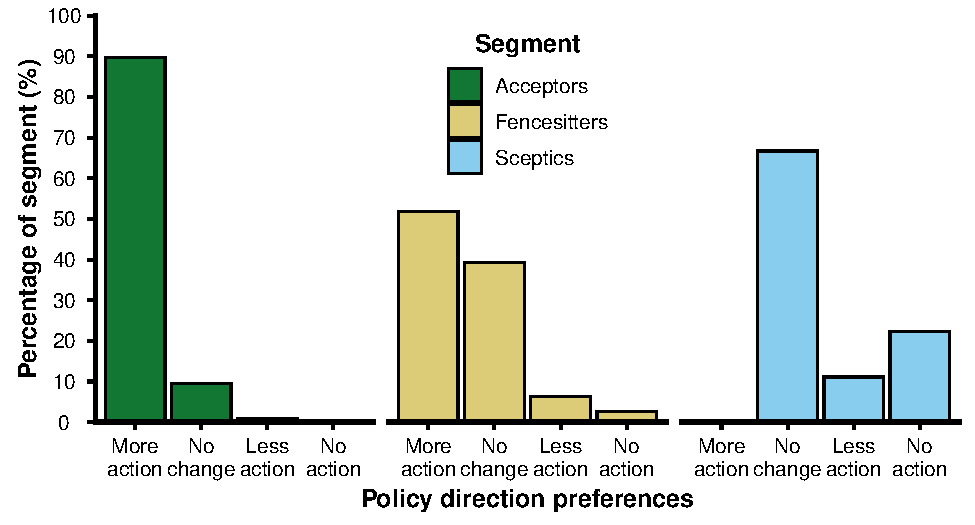
\includegraphics{analysis_files/figure-pdf/fig-policy-support-1.pdf}

}

\caption{\label{fig-policy-support}Policy direction preferences as a
function of segment.}

\end{figure}


  \bibliography{references.bib}


\end{document}
